%% 
%% Copyright 2007, 2008, 2009 Elsevier Ltd
%% 
%% This file is part of the 'Elsarticle Bundle'.
%% ---------------------------------------------
%% 
%% It may be distributed under the conditions of the LaTeX Project Public
%% License, either version 1.2 of this license or (at your option) any
%% later version.  The latest version of this license is in
%%    http://www.latex-project.org/lppl.txt
%% and version 1.2 or later is part of all distributions of LaTeX
%% version 1999/12/01 or later.
%% 
%% The list of all files belonging to the 'Elsarticle Bundle' is
%% given in the file `manifest.txt'.
%% 

%% Template article for Elsevier's document class `elsarticle'
%% with numbered style bibliographic references
%% SP 2008/03/01

%\documentclass[preprint,12pt]{elsarticle}

%% Use the option review to obtain double line spacing
%% \documentclass[authoryear,preprint,review,12pt]{elsarticle}
%%  \documentclass[2014,preprint,review,12pt]{elsarticle}

%% Use the options 1p,twocolumn; 3p; 3p,twocolumn; 5p; or 5p,twocolumn
%% for a journal layout:
% \documentclass[final,1p,times]{elsarticle}
%% \documentclass[final,1p,times,twocolumn]{elsarticle}
%% \documentclass[final,3p,times]{elsarticle}
%% \documentclass[final,3p,times,twocolumn]{elsarticle}

%% \documentclass[final,5p,times,twocolumn]{elsarticle}

%% For including figures, graphicx.sty has been loaded in
%% elsarticle.cls. If you prefer to use the old commands
%% please give \usepackage{epsfig}

%% The amssymb package provides various useful mathematical symbols

%% The amsthm package provides extended theorem environments
%% \usepackage{amsthm}

%% The lineno packages adds line numbers. Start line numbering with
%% \begin{linenumbers}, end it with \end{linenumbers}. Or switch it on
%% for the whole article with \linenumbers.
%% \usepackage{lineno}

%% Title, authors and addresses

%% use the tnoteref command within \title for footnotes;
%% use the tnotetext command for theassociated footnote;
%% use the fnref command within \author or \address for footnotes;
%% use the fntext command for theassociated footnote;
%% use the corref command within \author for corresponding author footnotes;
%% use the cortext command for theassociated footnote;
%% use the ead command for the email address,
%% and the form \ead[url] for the home page:
%% \title{Title\tnoteref{label1}}
%% \tnotetext[label1]{}
%% \author{Name\corref{cor1}\fnref{label2}}
%% \ead{email address}
%% \ead[url]{home page}
%% \fntext[label2]{}
%% \cortext[cor1]{}
%% \address{Address\fnref{label3}}
%% \fntext[label3]{}


%% use optional labels to link authors explicitly to addresses:
%% \author[label1,label2]{}
%% \address[label1]{}
%% \address[label2]{}

% % % % % % % % % % % % % % % % % % % % % % % % % % % % % % % % % % % % % % % % % % % % % % % % % %
% % % % Preamble
% % % % % % % % % % % % % % % % % % % % % % % % % % % % % % % % % % % % % % % % % % % % % % % % % %
\documentclass[preprint,5p,times]{elsarticle}
%\documentclass[2015,preprint,review,12pt]{elsarticle}
\usepackage{amssymb}
\usepackage{amsmath}
\usepackage{epsfig}
\usepackage{url}
\usepackage{float}
\usepackage{tabularx}
\usepackage{cancel}
\usepackage{booktabs}
\usepackage{subfigure}
\journal{International Journal of Impact Engineering}
\begin{document}
	% % % % % % % % % % % % % % % % % % % % % % % % % % % % % % % % % % % % % % % % % % % % % % % % % %
	% % % % Frontmatter (Authors/Abstract/Keywords)
	% % % % % % % % % % % % % % % % % % % % % % % % % % % % % % % % % % % % % % % % % % % % % % % % % %
	\begin{frontmatter}
		%\title{Numerical modelling of the structural response of welded materials under complex loading configurations. %panels subjected to air blast.
		%Part I: Numerical modelling}
		\title{Finite element based modelling of the structural response of welded materials in complex loading configurations. %panels subjected to air blast.
			Part II: Constitutive modelling considerations}
		\author[1]{A.J. Awang Draup \corref{cor1}}
		\ead{jefri.draup@postgrad.manchester.ac.uk}
		\author[1]{B.I. Rodgers}
		\author[1]{J.D Robson}
		\author[1]{P.B. Prangnell}
		\author[1]{Q.M. Li}
		\address[1]{The University of Manchester, Manchester, M13 9PL, UK}
		\author[2]{M.J. Lunt}
		\address[2]{DSTL, Porton, SP4 0JQ, UK}
		\cortext[cor1]{Corresponding author. Tel: +44 (0)161 306 3578 Ext. 2261}
		
		\begin{abstract}
			This two-part article presents the results of numerical  prediction and experimental studies which aim to determine the structural response of friction stir welded aluminium 2139-T8 subjected to complex loading configurations, and in particular, air blast loading. The aim of this work is to develop a numerical modelling methodology to allow detailed prediction of the local strain evolution across the weld zone as this has significant influence in relation to structural response and failure. In particular, the method allows local material property gradients, which are due to variation in strengthening mechanism arising from microstructural damage caused by thermal loading during the welding process, to be incorporated into a macro scale structural model. Part I details the methodology used to implement local material property gradients together with experimental evidence to verify the predicted structural response in a range of loading configurations. Part II provides an insight into the assumptions made in Part I with respect to high strain rate materials modelling across the weld zone and the associated evidence for the variation in strengthening mechanisms in the alloy. The combined work presented highlights the importance of accurate description of the variation in local material properties, particularly the work hardening rate, in determining the response of structures under blast loading.
		\end{abstract}
		
		\begin{keyword}
			%% keywords here, in the form: keyword \sep keyword
			Blast loading\sep Digital image correlation \sep Materials modelling \sep Finite element simulation \sep Materials characterisation
			%% PACS codes here, in the form: \PACS code \sep code
			%% MSC codes here, in the form: \MSC code \sep code
			%% or \MSC[2008] code \sep code (2000 is the default)
		\end{keyword}
		
	\end{frontmatter}
	
	% % % % % % % % % % % % % % % % % % % % % % % % % % % % % % % % % % % % % % % % % % % % % % % % % %
	% % % % Introduction
	% % % % % % % % % % % % % % % % % % % % % % % % % % % % % % % % % % % % % % % % % % % % % % % % % %
	\section{Introduction}
	%	\label{Intro}
	%	%
	%%	\begin{itemize}
	%%		\item context
	%%		\item What happened in Part I and how Part II fits in
	%%		\item The use of Johnson-Cook materials models in FE of FSW (no property variation apart from yield stress)
	%%		\item Material Properties and Microstructure and strengthening mechanism link
	%%		\item Summarise that this part is basically to understand how to apply materials modelling appropriately to FSW 2139-T8
	%%	\end{itemize}
	%	
	%	It is widely accepted that the mechanical properties of metals are linked to the material mircostructure and the strengthening mechanisms of the alloy. For heat treatable aluminium alloys, such as 2139-T8, the mechanisms which contribute to the strength of the alloy are: precipitate strengthening, solid solution strengthening, work hardening, and grain size refinement. Joining processes, such as Friction Stir Welding (FSW), induce significant transient temperature rise and plastic deformation through interaction of the work-piece with the welding tool. Whilst temperature rises in FSW remains below the melting point of aluminium, the combination of thermal and mechanical loading can induce diffusional  and recrystallisation processes which affect the material microstructure and, hence, the strengthening mechanisms of the welded material. As a result, there are large variations in material and  mechanical properties across a weld zone.
	%	
	%	In Finite Element based modelling, the use of Johnson-Cook material models is commonplace when simulating the non-linear response structures. However, since obtaining parameters locally within a weld can be expensive, a typical method for simplifying the material modelling process is to assume that there is only variation in yield stress across a weld. It is generally accepted that there may be significant variation in properties, such as the work hardening rate, across a weld. Structural modelling for the purposes of determining non-linear response can therefore be difficult and require careful calibration and interpretation.	In Part I of this study, a method for implementing material property gradients in macro scale FE models to simulate structural response of FSW 2139-T8 was developed. The method was shown to provide accurate quantitative prediction of strain evolution in structures under complex loading configurations including blast loading. However, the parameters for the material models across the weld were merely stated. 
	%	
	%	In this companion paper, a generalised semi-empirical method for determining the Johnson-Cook parameters across finite elements in a model of the weld zone is presented. In addition, observations of material microstructure are presented, which are used to justify the logical approach to assigning parameters. In theory, this method can be used to determine the effects of welding parameters on the Johnson-Cook parameters across a weld zone, though this has not been experimentally verified here. The application of this method requires a sound understanding of the physical metallurgy of the aluminium alloy 2139-T8.
	%	
	%	\subsection{Aluminium 2139-T8}
	%	\label{Intro2139T8} 
	%	Whilst there are many mechanisms contributing to the strength of an alloy, for age hardenable alloys, such as Al-Cu-Mg-Ag based 2139-T8, the predominant strengthening mechanism is due precipitate strengthening. Ternary Al-Cu-Mg alloys with low Cu:Mg ratios are known to lead to the formation of the $\text{Al}_2$CuMg based S' or S phases, whereas alloys with high Cu:Mg ratios lead to the formation of Cu GP zones and subsequently the $\text{Al}_2$Cu $\theta'$ phase. Above Cu:Mg ratios of approximately 5.6, the addition of trace amounts of Ag enhance the age hardening response and, additionally, promote the formation of $\text{Al}_2$Cu based precipitates ahead of S' and S phases; $\theta$ forms habitually on the $\text{\{100\}}_\mathrm{\alpha}$ and $\Omega$ forms habitually on the $\text{\{111\}}_\mathrm{\alpha}$. Under the appropriate heat treatment, the hexagonal plate-like $\Omega$ phase forms ahead of GP zones leading to high densities of the strengthening phase. In the T8 condition, the size and distribution of $\Omega$ phase is optimised to reduce dislocation motion, hence 2139 is considered to offer peak strength.
	%	\section{Alternative Introduction}
	It is widely accepted that the mechanical properties of metals are linked to the material microstructure and the strengthening mechanisms of the alloy. For age hardenable aluminium alloys, the mechanisms which contribute to the strength of the alloy include: precipitate hardening, solid solution strengthening, work hardening, and grain size refinement \cite{Shercliff1990a}.
	% but the most significant contribution to alloy strength is from precipitate hardening. 
	Upon age hardening, ternary Al-Cu-Mg alloys with low Cu:Mg ratios are known to lead to the formation of the $\text{Al}_2$CuMg based S' or S phases \cite{Bakavos2008}. In comparison, Al-Cu-Mg alloys with high Cu:Mg ratios lead to the formation of Cu GP zones and subsequently the $\text{Al}_2$Cu $\theta'$ phase; the addition of Ag promotes formation of the $\text{Al}_2$Cu based $\Omega$ phase \cite{Bakavos2008,Muddle1989,Nie2001}. The addition of trace amounts of Ag in ternary alloys with Cu:Mg ratios of above 5.6, such as 2139-T8, enhances the age hardening response and promotes the formation of $\text{Al}_2$Cu based precipitates ahead of S' and S phases \cite{Bakavos2008}. $\theta$ forms habitually on the $\text{\{100\}}_\mathrm{\alpha}$ and $\Omega$ forms habitually on the $\text{\{111\}}_\mathrm{\alpha}$ \cite{Elkhodary2011b}. Under the appropriate heat treatment, the hexagonal plate-like $\Omega$ phase forms ahead of GP zones leading to high densities of the strengthening phase \cite{Bakavos2008}. In the T8 condition, the size and distribution of $\Omega$ phase is optimised to reduce dislocation motion, hence 2139 is considered to offer peak strength.
	
	Joining processes, such as Friction Stir Welding (FSW), induce significant transient temperature rise and plastic deformation through interaction of the welding tool with the work-piece \cite{Mishra2005,Robson2006a}. Whilst temperature rises in FSW remains below the melting point of aluminium, the combination of thermal and mechanical loading can induce diffusional and recrystallisation processes in the work-piece \cite{Sato1999,Sato1999a,Sato2001}. FSW is known to cause phenomena such as precipitate coarsening; local dissolution of precipitates; recovery and recrystallisation. This leads to the formation of meso-scale regions across the weld known as the nugget, the Thermo-Mechanically Affected Zone (TMAZ), and the Heat Affected Zone (HAZ). The combined thermal and plastic deformation effects on the material microstructure alter the local material properties in welded structures \cite{Sato1999,Sato1999a,Sato2001,Mishra2005}. As a result, there are large gradients in material and mechanical properties across a weld zone \cite{Mahoney1998}. 
	
	In Finite Element based modelling, the use of Johnson-Cook constitutive models is commonplace when simulating the non-linear response structures \cite{Grujicic2011,McWilliams2013}. However, since obtaining parameters locally within a weld is difficult \cite{Genevois2006}, the typical method for defining the constitutive model parameters across the weld zone is to assume that there is only variation in yield stress across a weld \cite{Grujicic2011,McWilliams2013}. It is generally accepted that there may be significant variation in properties, such as the work hardening rate, across a weld \cite{Grujicic2012,McWilliams2013,Sullivan2011}. Thus, determining the non-linear response of welds can be difficult and require careful calibration and interpretation.	In Part I of this study, a method for implementing material property gradients in macro scale FE models to simulate structural response of FSW 2139-T8 was developed. The method was shown to provide accurate quantitative prediction of strain evolution in structures under complex loading configurations including blast loading. However, the constitutive model parameters for elements across the weld zone were merely stated. 
	
	In this companion paper, the Johnson-Cook parameters for the different regions of a weld are estimated by measuring the mechanical properties from simulated weld material (\S\ref{ModellingProcess}) which is representative of a generalised weld condition. The variation in parameters is related to observations of the microstructure using methods described in \S\ref{EM}. Together with theory presented by Shercliff \cite{Shercliff1990,Shercliff1990a}, the Johnson-Cook parameters across general welding condition can be defined using the method described in \S\ref{RADJCModel} 
	%	
	%	In this companion paper, a generalised semi-empirical method for determining the Johnson-Cook parameters across a weld cross section is presented. The Shercliff method is used to 
	%	The stress-strain response of material heat treated to simulate the different regions of a weld normalised for any weld condition is measured empirically. Johnson-Cook parameters 
	%	The Shercliff model for predicting the post weld hardness profile is used to define regions in the weld where there are distinct changes in microstructure. In this study, the Johnson-Cook parameters from different regions of a weld are estimated by measuring the mechanical properties from simulated weld material (\S\ref{ModellingProcess}). The variation in parameters is related to observations of the microstructure using methods described in \S\ref{EM}. The application of the developed constitutive models is described in Part I, the companion paper. 
	%	In addition, observations of material microstructure are presented, which are used to justify the logical approach to assigning parameters. In theory, this method can be used to determine the effects of welding parameters on the Johnson-Cook parameters across a weld zone, though this has not been experimentally verified here. The application of this method requires a sound understanding of the physical metallurgy of the aluminium alloy 2139-T8.
	%	
	% % % % % % % % % % % % % % % % % % % % % % % % % % % % % % % % % % % % % % % % % % % % % % % % % %
	% % % % Materials Modelling
	% % % % % % % % % % % % % % % % % % % % % % % % % % % % % % % % % % % % % % % % % % % % % % % % % %
	\section{Background Theory}
	\label{Modelling}
	In this study, a model developed originally by Shercliff \cite{Shercliff1990,Shercliff1990a} and adapted by Robson \cite{Robson2006a} was used to gain an understanding of the effect of the welding process on the properties of 2139-T8. The model used to interpret microstructural variation across the weld and can be used to help identify a logical method for assigning constitutive model parameters in weld cross sections (\S\ref{RADJCModel}). The model was also used to recreate ``simulated weld material" (\S\ref{EMSimulateMicrostructure})in order to measure the mechanical properties across the weld. 
	\subsection{Process Modelling}
	\label{ModellingProcess}
	%	Shercliff Model theory; How it can be used to predict post-weld hardness (an indicator of YS); and how it can be used to simulate microstructure (put in a table of heat treatments) and thus examine how mechanical properties vary in relation to microstructure \& strengthening mechanism.
	Shercliff et al. \cite{Shercliff1990,Shercliff1990a} originally developed a model to predict the as-welded hardness distribution heat treatable aluminium alloys. The model assumes that changes to strength during the thermal cycle from welding are related to the volume fraction of precipitates in the material, which is further assumed to have linear relationship with hardness (equation \ref{eq1}). The model assumes that any softening is caused by dissolution of strengthening precipitates which is modelled using a 2-dimensional diffusion model of dissolution (equation \ref{eq2}). Dissolution behaviour is normalised to a calibrated reference temperature by experimental measurement of the time required to cause complete softening, and hence complete precipitate dissolution, at that temperature. This normalisation procedure eliminates any dependence of the diffusion model on precipitate geometry and can be used to estimate the time for complete dissolution to occur at any temperature (equation \ref{eq3}). Since the model assumes isothermal heat treatments, the transient temperature profiles during welding are accounted for by using equation \ref{eq4}. Details of the Shercliff model \cite{Shercliff1990,Shercliff1990a} and adaptations by Robson \cite{Robson2006a} can be found elsewhere, therefore only a brief description is given here.
	\begin{equation}
	\label{eq1}
	X_p = \frac{HV-HV_{min}}{HV_{max}-HV_{min}}
	\end{equation}
	\begin{equation}
	\label{eq2}
	X_p =1-\bigg(\frac{t}{t_1^{*}}\bigg)^{\frac{1}{2}}
	\end{equation}
	\begin{equation}
	\label{eq3}
	t_1^{*} =t_{r1}e^{\bigg\{\bigg(\frac{Q_{eff}}{R}\bigg)\bigg(\frac{1}{T}-\frac{1}{T_r}\bigg)\bigg\}}
	\end{equation}
	\begin{equation}
	\label{eq4}
	\bigg(\frac{t}{t_1^{*}}\bigg)_{eff} =\int_{0}^{t}\frac{dt}{t_1^{\text{*}}}
	\end{equation}
	The Shercliff model can be used, therefore, to predict the as-welded hardness distribution in a weld. Contribution to strengthening from post-weld natural aging can be accounted for by empirical measurement of the natural aging response (hardness) \cite{Robson2006a}. Thus, if one assumes a linear relationship of yield stress with hardness (equation \ref{eq6}), the model can be used to predict the post-weld yield stress. Indeed, several studies have shown that the model has bee successfully used to predict the post-weld strength distribution across FSW 2xxx, 6xxx, and 7xxx series aluminium alloys \cite{Shercliff2005,Robson2006}. Two observations can be made of the Shercliff model, which are used in this study:
	\begin{enumerate}
		\item Typically, the as-welded strength profile and the post natural aging strength profiles have characteristic ``flat trough U-shape" and ``W-shape" profiles respectively. It can be shown mathematically that the region of the weld enveloped by the flat trough of the U-shape and the region in between the two minima of the W-shape coincide with the positions in the weld cross section where the sum of equation \ref{eq4} is equal to 1. Hence, from the hardness profile, we can infer the geometric boundaries in the weld cross section where we can assume that locally, the strengthening precipitates have undergone full dissolution according to equation \ref{eq2}. %This theoretical state of dissolution will be used in \S\ref{RADJCModel} when logically assigning Johnson-Cook parameters across the weld zone.
		
		\item Whilst the Shercliff model is designed to predict post-weld hardness from knowledge of the local weld thermal cycle, it can be used in reverse to calculate equivalent isothermal heat treatments which can be used to heat treat parent material to the equivalent hardness of any position across the weld \cite{Shercliff2005,Sullivan2011}. In this way, it is possible to generate monolithic material from 2139-T8 in the as-received condition to ``simulate" the local microstructure anywhere in the weld cross section. Thus, mechanical properties of local weld structure can be estimated through mechanical testing of simulated weld material as discussed in \S\ref{EMSimulateMicrostructure}. 
	\end{enumerate}
	
	\subsection{Constitutive Modelling}
	\label{ModellingMaterials}
	%	What is JC model?
	%	What does it do?
	%	Its use in FE of welds?
	%	How do we intend to use it?
	%	Disadvantages of it?
	The Johnson-Cook constitutive model is a powerful tool for modelling the non-linear response of materials as it can capture the effects of strain rate and thermal sensitivity in addition to the quasi-static response of a material. Johnson-Cook constitutive models are frequently used to model the dynamic response of materials and structures under transient loading \cite{Grujicic2009,Grujicic2011a,Dey2007}. Their widespread use is linked to their ability to capture bulk properties over a range of conditions. The Johnson-Cook model describes the flow stress using the relationship using equation \ref{eq5}:
	\begin{equation}
	\label{eq5}
	\sigma = \bigg( A + B\epsilon^n_{p} \bigg)\; \bigg(1 +C\,\text{ln}\bigg(\frac{\dot{\epsilon}_{p}}{\dot{\epsilon}_{p0}}\bigg)\bigg)\; \bigg(1-\bigg(\frac{T-T_0}{T_m-T_0}\bigg)^m\bigg)
	\end{equation}	
	Where A is the quasi-static yield stress, B is the strength coefficient, n is the work hardening rate, C is the strain rate sensitivity, and m is the thermal sensitivity. As described by Johnson and Cook, these parameters are obtained empirically through experiments which approximately isolate quasi-static response, dynamic response, and thermal response respectively. 
	
	Unfortunately, extensive experimental work is required in order to develop complete set of parameters for any particular material \cite{Johnson1983c}. 
	For material in the weld, due to the property gradients induced by the transient welding process, the added complication of obtaining representative specimens makes it difficult to measure local properties \cite{Genevois2006}.
	As a result, it is often the case that parameters are inferred from literature or are assumed to remain unchanged across the weld. In studies by McWilliams \cite{McWilliams2013} and Grujicic \cite{Grujicic2011a}, which apply the ``lumped-mass" method described in Part I, it is assumed that the only parameter in equation \ref{eq5} that varies across the weld zone is the A parameter. This simplification is commonly made despite wide comprehensive evidence of variance in properties, particularly the work hardening rate, across a weld. 
	
	%	In this study, the Johnson-Cook parameters from different regions of a weld are estimated by measuring the mechanical properties from simulated weld material (\S\ref{ModellingProcess}). The variation in parameters is related to observations of the microstructure using methods described in \S\ref{EM}. The application of the developed constitutive models is described in Part I, the companion paper. 
	%	
	%	Other disadvantages of this type of model include:
	%	
	%	\begin{itemize}
	%		\item Quasi-static properties are fully coupled to strain rate and thermal effects
	%		\item For materials such as steel, the model does not allow for a lower yield point
	%		\item Portevin-Le Chatelier effect can not be incorporated
	%		\item Time consuming to develop parameters
	%	\end{itemize}
	%	Despite these shortcoming, the Johnson-Cook constitutive model has been successfully applied to model the non-linear response of materials under complex loading configurations. In this study, the Johnson-Cook model is used to simu
	%	
	%TODO Use disadvantages in the discussion of results
	
	% % % % % % % % % % % % % % % % % % % % % % % % % % % % % % % % % % % % % % % % % % % % % % % % % %
	% % % % Experimental Methods
	% % % % % % % % % % % % % % % % % % % % % % % % % % % % % % % % % % % % % % % % % % % % % % % % % %
	\section{Experimental Methods}
	\label{EM}
	\subsection{Weld Microstructure}
	\label{EMWeldMicrostructure}
	Bead on plate FSW was carried out on 2139-T8 alloy where the work-piece dimensions are 150x300x38 mm. Welding was carried out with a conventional tool with triflat pin set at a 2$^\circ$ rake angle. The tool dimensions were: 34 mm shoulder diameter; 2$^\circ$ shoulder concave angle; 18 mm pin root diameter; 20 mm pin height; 10 mm pin tip diameter. The weld settings were: 150 $\text{mm}\!\cdot\!\text{min}^{-1}$ traverse speed; 500 RPM rotation speed; 55 kN downforce. The welds were carried out with the tool in force control mode. A regular line profile of hardness measurements in the weld cross section was made across the weld centreline; hardness indentations were spaced every 1 mm at a position 10 mm from the top surface of the weld. Samples were prepared for TEM studies (\S\ref{EMTem}) from a cross section in the centre of the weld and in positions 10 mm from the top surface of the weld. Samples for microscopy (\S\ref{EMTem} and \S\ref{EMSem}) were taken from the positions indicated in figure \ref{fig:TEMpositions} and are representative of the parent material ($x=50$ mm); the outer region of the HAZ ($x=50$ mm); the inner region of the HAZ ($x=50$ mm); the TMAZ ($x=50$ mm); and the weld nugget ($x=50$ mm). %TODO check the dimensions of these positions
	\begin{figure}[h!]
		\centering
		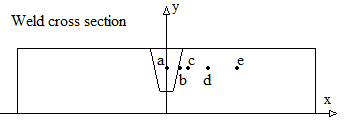
\includegraphics[width=1\linewidth]{TEMpositions}
		\caption[Dogbone]{Locations in the weld regions where samples are sectioned and representative of a) the nugget b) the TMAZ c) the inner HAZ d) the outer HAZ and e) the parent material.}	
		\label{fig:TEMpositions}
	\end{figure} 
	\subsection{Simulated Microstructure}
	\label{EMSimulateMicrostructure}
	In accordance with the Shercliff method \cite{Shercliff1990,Shercliff1990a} described in \S\ref{ModellingProcess}, 2139-T8 material for each experimental method was heat treated according to table \ref{tab:HeatTreatments}. All samples, such as dog-bone and compression specimens, were machined prior to heat treatment, and quenched in room temperature water. The samples are heat treated to be equivalent as the positions indicated in figure \ref{fig:TEMpositions}. However, representative nugget material was obtained by machining specimens for mechanical testing from the nugget region of an actual weld using the conditions described in \S\ref{EMWeldMicrostructure}
	
	\begin{table}[htbp]
		\centering
		\caption{Isothermal heat treatments applied to as-received 2139-T8 in order to simulate the microstructure across and actual weld.}
		\resizebox{\columnwidth}{!}{%
			\begin{tabular}{@{}cccc@{}}
				\toprule
				\begin{tabular}[c]{@{}c@{}}Equivalent Position \\ in Weld\end{tabular} & \begin{tabular}[c]{@{}c@{}}Vickers Hardness\end{tabular} & \begin{tabular}[c]{@{}c@{}}Temperature ($^\circ$C)\end{tabular} & \begin{tabular}[c]{@{}l@{}}Time (Minutes) \\\end{tabular} \\ \midrule
				Base Metal & 175 & N/A     & N/A \\
				HAZ Outer & 150 & 275   & 36 \\
				HAZ Inner & 120 & 375   & 21 \\
				Nugget & 120 & N/A   & N/A \\
				\bottomrule 
			\end{tabular}
		}
		\label{tab:HeatTreatments}%
	\end{table}%
	
	%TODO insert and reference table
	\subsection{Quasi-Static Room Temperature Tensile Testing}
	\label{EMTensileRT}
	The purpose of testing is to obtain a measure of the A, B, and n parameters across all regions of the weld zone, as defined by equation \ref{eq5}. Dogbone specimens (figure \ref{fig:TensileSpecimen}) were machined from as-received 2139-T8 rolled sheet with 1.6 mm gauge thickness. Samples were heat treated according to the regime described in table \ref{tab:HeatTreatments} and subsequently tested in an Instron 5569 electromechanical load frame fitted with a 50 kN load cell. Samples were tested in the strain rate regime $10^{-4}$ s$^{-1}$ by setting the cross-head displacement rate to 2 $\text{mm}\!\cdot\!\text{min}^{-1}$. Testing was carried out in accordance with BS6892-1:2009. 
	\begin{figure}[h!]
		\centering
		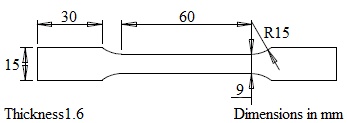
\includegraphics[width=1\linewidth]{dogbone}
		\caption[Dogbone]{Dimensions of tensile specimens used for tensile testing both at room temperature and high temperatures.}	
		\label{fig:TensileSpecimen}
	\end{figure} 
	\subsection{Quasi-Static High Temperature Tensile Testing}
	\label{EMTensileHT}
	The purpose of testing is to obtain a measure of the m parameter across all regions of the weld zone, as defined by equation \ref{eq5}. Dogbone specimens (figure \ref{fig:TensileSpecimen}) were machined from as-received 2139-T8 rolled sheet with 1.6 mm gauge thickness. Samples were heat treated according to the regime described in table \ref{tab:HeatTreatments} and subsequently tested in a Gleeble 3500 thermal-mechanical test system fitted with a 100 kN load cell. Samples from each weld region were tested after an initial heating ramp and soak time; testing was carried out in the strain rate regime $10^{-4}$ s$^{-1}$ by setting the cross-head displacement rate to 2 $\text{mm}\!\cdot\!\text{min}^{-1}$. Testing was carried out in accordance with BS6892-2:2011, with the exception that the soak time during testing was less than the mandatory 10 minutes. This was because 2139-T8 alloy undergoes solid state transformation processes at the test temperatures in table \ref{tab:HighTempPlan}, hence, soak time was minimised to mitigate these effects. 
	\begin{table}[htbp]
		\centering
		\caption{High temperature test plan used to test samples from simulated weld regions defined in \S\ref{EMSimulateMicrostructure}.}
		\begin{tabularx}{\columnwidth}{X*{5}{c}} 
			\toprule
			Test Temperature ($^\circ$C) & 100   & 200   & 300   & 400 \\
			\midrule
			Heat Ramp ($^\circ$Cs$^{-1}$) & 20    & 20    & 20    & 20 \\
			Soak Time (s) & 5     & 5     & 5     & 5 \\
			\bottomrule
		\end{tabularx}%
		\label{tab:HighTempPlan}%
	\end{table}%
	%	
	%	\begin{table}[htbp]
	%		\centering
	%		\caption{High temperature test plan used to test samples from simulated weld regions defined in \S\ref{EMSimulateMicrostructure}.}
	%		\resizebox{\columnwidth}{!}{%
	%			\begin{tabular}{@{}ccccc@{}}
	%				\toprule
	%				\begin{tabular}[c]{@{}c@{}}Test Temperature ($^\circ$C)\end{tabular} & \begin{tabular}[c]{@{}c@{}}100 \end{tabular} & \begin{tabular}[c]{@{}c@{}}200\end{tabular} & \begin{tabular}[c]{@{}l@{}}300\end{tabular} & \begin{tabular}[c]{@{}l@{}}400\end{tabular} \\ \midrule
	%				Heat Ramp ($^\circ$Cs$^{-1}$) & 20    & 20    & 20    & 20 \\
	%				Soak Time (s) & 5     & 5     & 5     & 5 \\  \bottomrule
	%			\end{tabular}
	%		}
	%		\label{tab:High}%
	%	\end{table}%
	
	\subsection{High Strain Rate Room Temperature Compression Testing}	
	\label{EMKolsky}
	The purpose of testing is to obtain a measure of the C parameter across all regions of the weld zone, as defined by equation \ref{eq5}. Cylindrical specimens were machined from 38 mm gauge as-received 2139-T8 and heat treated to simulate weld material as described in \S\ref{EMSimulateMicrostructure}. A Kolsky bar apparatus, setup as described Gray%TODO add reference of ASM handbook
	, was used to test samples across a wide range of strain rates as described by table \ref{tab:HighStrainRate}. All bars were machined from 20 mm diameter mild steel rods, where the measured speed of sound was approximately 3300 ms$^{-1}$.The striker bar was machined to a length of 250 mm; the incident bar to 1000 mm; and the transmitter to 1500 mm. 
	
	\begin{table}[htbp]
		\centering
		\caption{High strain rate test plan used to test samples from simulated weld regions defined in \S\ref{EMSimulateMicrostructure}.}
		\resizebox{\columnwidth}{!}{%
			\begin{tabular}{@{}cccc@{}}
				\toprule
				\begin{tabular}[c]{@{}c@{}}Sample \\Diameter (mm)\end{tabular} & \begin{tabular}[c]{@{}c@{}}Sample \\Length (mm)\end{tabular} & \begin{tabular}[c]{@{}c@{}}Striker Velocity\\ (ms$^{-1}$)\end{tabular} & \begin{tabular}[c]{@{}l@{}}Estimated Test\\ Strain Rate (s$^{-1}$)\end{tabular} \\ \midrule
				6.00                                                           & 6.00                                                         & 6.00                                                         & 600                                                                        \\
				6.00                                                           & 4.00                                                         & 10.00                                                         & 1500                                                                       \\
				5.00                                                           & 2.00                                                         & 10.00                                                         & 3500                                                                       \\ \bottomrule
			\end{tabular}
		}
		\label{tab:HighStrainRate}%
	\end{table}%
	%\begin{tabul
	\subsection{Transmission Electron Microscopy}
	\label{EMTem}
	High resolution imaging of 2139-T8 was carried out using both a Philips CM200 and an FEI Tecnai 30 Transmission Electron Microscope (TEM). TEM analysis was required to observe the response of plate-like $\Omega$ strengthening phase to FSW as $\Omega$ is of the order 10$^2$ nm in diameter and 10$^1$ nm in thickness. Samples were prepared from regions in the cross section of an actual weld (see figure \ref{fig:TEMpositions} \S\ref{EMWeldMicrostructure}), including the nugget; TMAZ; inner region of the HAZ; outer region of the HAZ; and the parent material. Samples from ``simulated" weld material were also prepared by heat treating 38 mm gauge 2139-T8 in the as-received condition as specified in table \ref{tab:HeatTreatments} in order to compare actual microstructure to simulated microstructure. Samples were prepared firstly by grinding material to a thickness of 180 $\mu$m and subsequently punching 3 mm diameter discs. The discs were electropolished in using a 30\% by volume nitric acid and methanol solution at $-30^\circ$C. During imaging, the electron beam was aligned with the $<\!211\!>$ zone axis in order to view the hexagonal, plate-like $\Omega$ precipitates edge on, as they form habitually along the \{111$\}_\alpha$.
	%TODO Put in beam settings (Brightfield mode, how many kEv etc.)
	\subsection{Scanning Electron Microscopy}
	\label{EMSem}
	An Ultra-55 FEG-SEM fitted with an Electron Back Scatter Diffraction (EBSD) probe was used to carry out micro-texture, and grain size analysis across FSW 2139-T8. EBSD patterns were produced with the microscope operating 20 kV; an aperture setting of 120 $\mu$m HC; and a working distance of 12 mm. Samples from the positions indicated in figure \ref{fig:TEMpositions} were prepared for analysis by systematic grinding and electro-polishing. Analysis was carried out using Oxford HKL Channel-5 software\footnote{All sample preparation and microscopy were carried out externally by Constellium (France), whilst data analysis was performed at the University of Manchester.}.
	
	% % % % % % % % % % % % % % % % % % % % % % % % % % % % % % % % % % % % % % % % % % % % % % % % % %
	% % % % Results and Discussions
	% % % % % % % % % % % % % % % % % % % % % % % % % % % % % % % % % % % % % % % % % % % % % % % % % %
	\section{Results and Discussion}
	\label{RAD}
	\subsection{Microstructural Observations}
	\label{RADMicrostructure}
	It is widely known that FSW leads to the development of meso-scale features in metals: the nugget, TMAZ, and HAZ \cite{Mishra2005}. The purpose of this study is to examine how the FSW process affects the local microstructure in 2139-T8. Furthermore, it is the purpose to determine if any particular microstructural features may require consideration when modelling non-linear plastic behaviour.
	\subsubsection{Precipitates}
	\label{RADMicrostructurePrecipitates}
	
	
	\begin{figure*}[h!t]
		\subfigure[Base Metal]{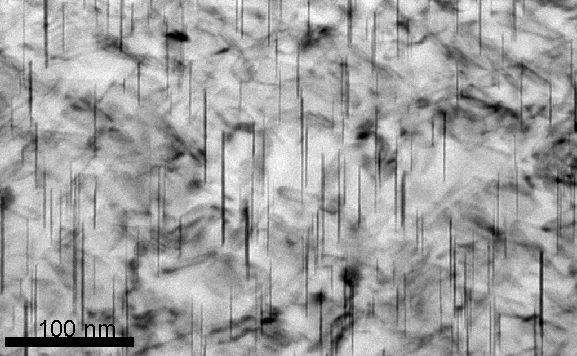
\includegraphics[width=1\columnwidth]{CROPBaseMetalTEMBar}}\hfill
		\subfigure[HAZ Outer]{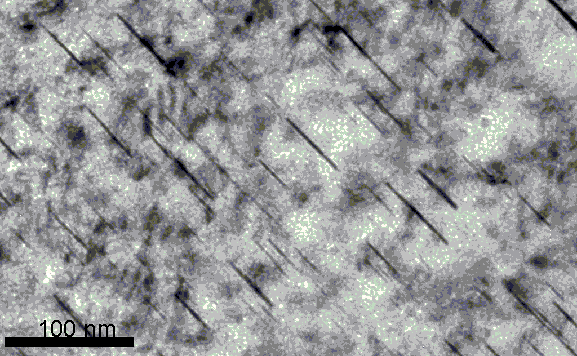
\includegraphics[width=1\columnwidth]{CROPHAZOuterTEMBar}}\hfill
		\subfigure[HAZ Inner]{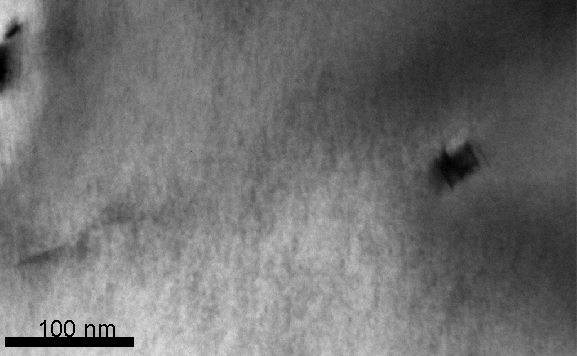
\includegraphics[width=1\columnwidth]{CROPHAZInnerTEMBar}}\hfill
		\subfigure[TMAZ]{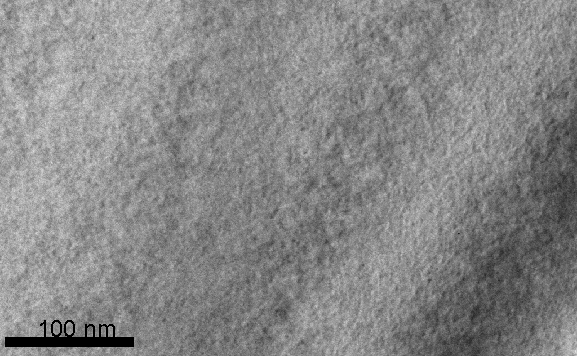
\includegraphics[width=1\columnwidth]{CROPTMAZTEMBar}}\hfill
		\subfigure[Nugget]{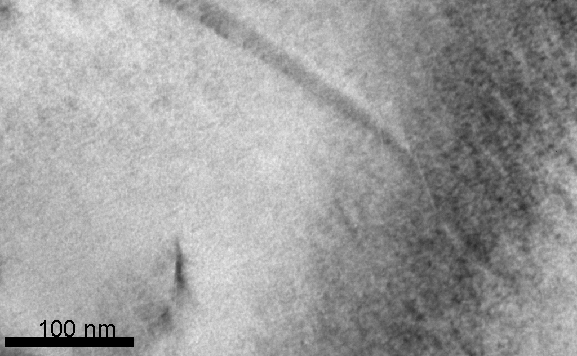
\includegraphics[width=1\columnwidth]{CROPNuggetTEMBar}} \centering
		\caption{TEM observation of 2139-T8 with the electron beam aligned with $<211>$ pole axis in all images. All hexagonal plate-like $\Omega$ precipitates appear as straight lines, as they are viewed edge on.}
		\label{fig:TEM}
	\end{figure*}
	
	Figure \ref{fig:TEM} shows the local distribution of $\Omega$ phase across the weld region. In the parent material, the controlled aging process leads to formation of hexagonal plate like precipitates which are approximately 50 nm in diameter and 2 nm thick. The precipitates are extremely finely distributed with perpendicular spacing estimated at approximately 10 nm. From observation, it is clear that the dominant feature of the parent material on this fine scale is the $\Omega$ phase and it is unsurprising that the strength of 2139-T8 is attributed to the $\Omega$ phase \cite{Cho2006}. 
	
	In the outer regions of the HAZ, where peak temperatures are relatively low, the $\Omega$ precipitates are much coarser and appear to be shorter, thicker, and more widely distributed in comparison with the parent material. The precipitate dimensions are approximately 30 nm in length, 3 nm in thickness, and the perpendicular spacing increases to approximately 30 nm. The thermal cycle has allowed diffusional processes to cause over-aging of the precipitates, thereby altering the precipitate dimensions and distribution. Nevertheless, on the fine scale of figure \ref{fig:TEM}, the $\Omega$ phase remains the dominant feature and is likely to contribute most significantly to the local strength in the alloy. It is possible that some of the $\Omega$ phase has dissolved into solution thereby enhancing the contribution from solid solution strengthening. However, according to Shercliff \cite{Shercliff1990a}, if precipitates are over-aging from peak condition, the relative contribution from solid solution strengthening remains low.
	
	In the inner region of the weld zone (inner HAZ, TMAZ and nugget), where temperatures are much higher, the $\Omega$ phase appears to have gone fully into solution on the fine scale of figure \ref{fig:TEM}. In these regions, it is conjectured that the local alloy strength may be attributed to the formation of GP zones upon natural aging, solid solution strengthening from dissolved $\text{Al}_2$Cu, or from grain refinement. It is likely that the different contributors to alloy strength in the inner regions of the weld are comparatively as significant as each other. This is in line with theory on age hardening in aluminium alloys presented by Shercliff \cite{Shercliff1990a}. In addition, since the region has undergone an uncontrolled transient thermal cycle from the welding process the $\Omega$ phase is unlikely re-precipitate out post welding; the age hardening heat treatment is finely controlled to induce the formation of $\Omega$ phase \cite{Bakavos2008}. On this local scale, it is clear that $\Omega$ phase does not contribute significantly to strengthening in the alloy in the inner regions of the weld. 
	
	In the TEM images of the parent material and the outer HAZ, there is additional diffraction contrast beyond that caused by the strengthening $\Omega$ phase. This may be due to the presence of dislocation structures, which would have been generated during the alloy processing route, or due to additional phases in the material. In the images of the inner HAZ, TMAZ, and nugget, there is little in the way of diffraction contrast; this demonstrates an absence of dislocation structures in the material. The absence of dislocation structures in the inner regions of the weld is likely to be caused by recovery and recrystallisation process which cause annihilation of dislocations. There is, therefore, likely to be an effect on the work hardening rate in the inner regions of the weld.
	
	%	Figure \ref{fig:TEM} shows the local distribution of $\Omega$ phase in the parent material and it is clear that the prevalence of the precipitate on this local scale contributes significantly to the strengthening mechanism of the alloy. 
	%	Figurexx shows the $\Omega$ phase in the outer regions of the HAZ, where peak temperatures are relatively low. The precipitates are much coarser and appear to be shorter, thicker, and more widely distributed. The precipitate dimensions are approximately 30 nm in length, 3 nm in thickness, and the perpendicular spacing increases to approximately 30 nm. The thermal cycle has allowed diffusional processes to cause over-aging of the precipitates. Hence, the precipitates are much coarser and more widely distributed. Nevertheless, on the scale of figureXX the $\Omega$ phase remains the dominant feature and contributes to the strengthening mechanism locally in the alloy. Though it is possible that some of the $\Omega$ phase dissolves into solution and hence contribution from solid solution strengthening is enhanced. However, according to Shercliff, if precipitates are over-aging from peak condition, the relative contribution from solid solution strengthening remains low.
	%	In the inner region of the weld zone (inner HAZ, TMAZ and nugget), where temperatures are much higher, the $\Omega$ phase appears to have gone fully into solution on the scale indicated in figureXX. In these regions, it is likely that solid solution strengthening is comparatively as significant as other strengthening mechanisms in the alloy. This is in line with theory on age hardening in aluminium alloys presented by Shercliff. In addition, since the region has undergone an uncontrolled transient thermal cycle from the welding process the $\Omega$ phase does not re-precipitate out post welding. On this local scale, it is clear that $\Omega$ phase does not contribute significantly to strengthening in the alloy in these inner regions. It is likely that other features from natural aging, such as the formation of GP zones or grain size refinement, contribute to strengthening.
	%	
	
	%TODO Choose good images from TEM hopefully any that show dislocation loops as well as precipitates
	\subsubsection{Grains}
	\label{RADMicrostructureGrains}
	The HAZ and parent material appear to have similar grain structure. Equivalent grain diameter is approximately of the order of 10$^2$ $\mu$m and grains have elongated, pancake like structure, which is typical of rolled material. 
	The TMAZ region demonstrates two types of grain structure: the first has grains similar in size to the parent material but subjected to large deformation whilst the second has much smaller equiaxed grains. The equivalent grain diameter reported in table \ref{tab:Grains} is an average of these two grain structures, hence, it is lower than that of the parent material. This may be because the large proportion of fine grains skews the calculation of the average grain diameter. However, on average, the equivalent diameter of the TMAZ approaches that of the parent material and HAZ (10$^2$ $\mu$m).
	In the nugget region, the grains have a fine equiaxed structure; grain refinement in this region is approximately one order of magnitude (10$^1$). Due to the large plastic deformation and transient frictional heating due to interaction with the tool, it is likely that this region has undergone dynamic recrystallisation.
	In line with observations by Sato and Preuss, grain refinement is only significant in the nugget region.
	\begin{table}[htbp]
		\centering
		\caption{Observed microstructural characteristics in the distinct weld zones of FSW 2139-T8.}
		\resizebox{\columnwidth}{!}{%
			\begin{tabular}{@{}ccc@{}}
				\toprule
				\begin{tabular}[c]{@{}c@{}}Weld Region\end{tabular} & \begin{tabular}[c]{@{}c@{}}Equivalent \\diameter ($\mu$m)\end{tabular} & \begin{tabular}[c]{@{}c@{}}Observations\end{tabular}\\ 
				\midrule
				Base Metal & 117   & Rolled grains \\
				HAZ   & 122   & Rolled grains \\
				TMAZ  & 90    & \begin{tabular}{c}Deformed rolled grains,  \\Regions of diffuse recrystallisation \end{tabular} \\ 
				Nugget & 24    & Fine, equiaxed grains \\
				\bottomrule
			\end{tabular}
		}
		\label{tab:Grains}%
	\end{table}%
	
	\subsubsection{Micro-Texture}
	\label{RADMicrostructureTexture}
	In this study, material parameters for Johnson-Cook constitutive models are obtained experimentally from 2139-T8 from as-received material in a range of gauge thickness ($1.6 \leq t \leq 38 \text{mm}$). Since aluminium can exhibit anisotropy due to texture, EBSD studies were carried out to determine if texture development was significant due to either the welding process or the reduction of material gauge thickness by rolling. This helps to determine if the effects of texture development influences the experimentally obtained parameters of the constitutive models.
	\begin{figure*}[h!t]
		\subfigure[Base Metal (1.6 mm gauge thickness)]{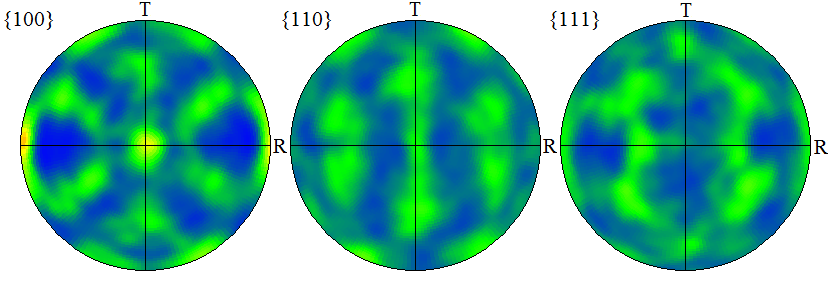
\includegraphics[width=1\columnwidth]{EDSBthingaugeC2}} \hfill
		\subfigure[Base Metal (12.7 mm gauge thickness)]{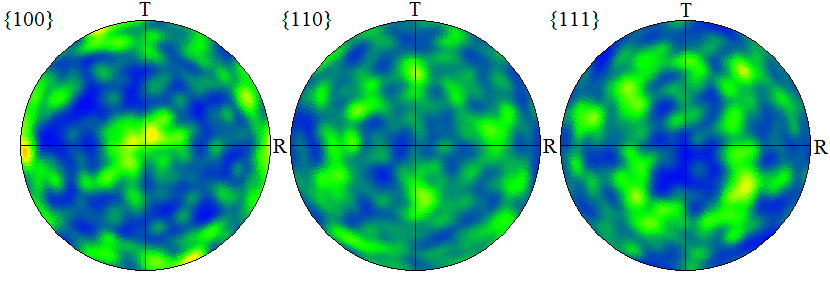
\includegraphics[width=1\columnwidth]{EDSBmediumgaugeC2}}\hfill
		\subfigure[Base Metal (38 mm gauge thickness)]{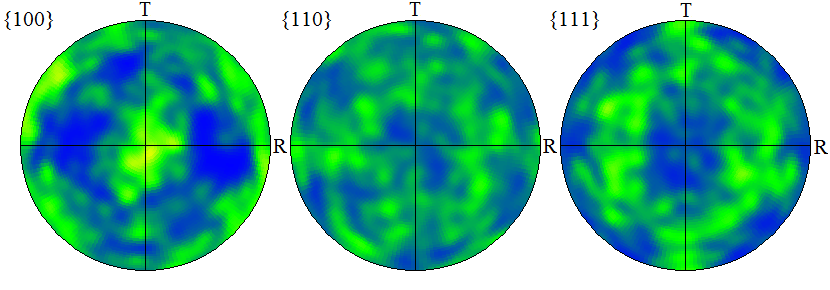
\includegraphics[width=1\columnwidth]{EDSBthickgaugeC2}}\hfill
		\subfigure[HAZ (38 mm gauge thickness)]{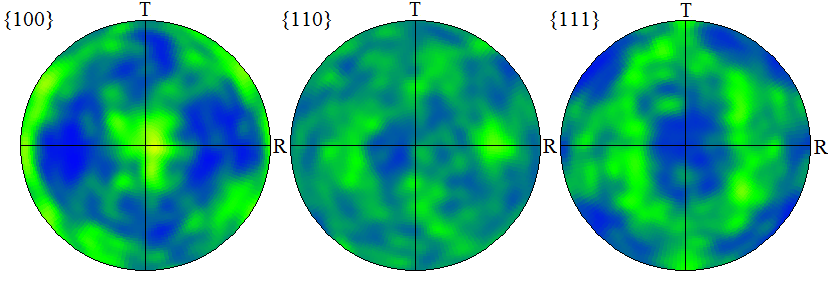
\includegraphics[width=1\columnwidth]{EDSBthickgaugeHAZC2}}\hfill
		\subfigure[TMAZ (38 mm gauge thickness)]{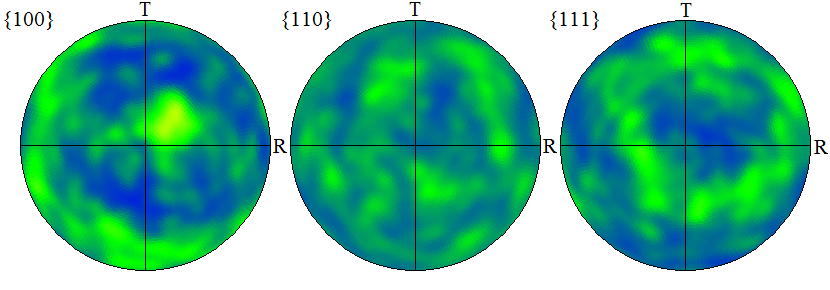
\includegraphics[width=1\columnwidth]{EDSBthickgaugeTMAZC2}}\hfill
		\subfigure[Nugget (38 mm gauge thickness)]{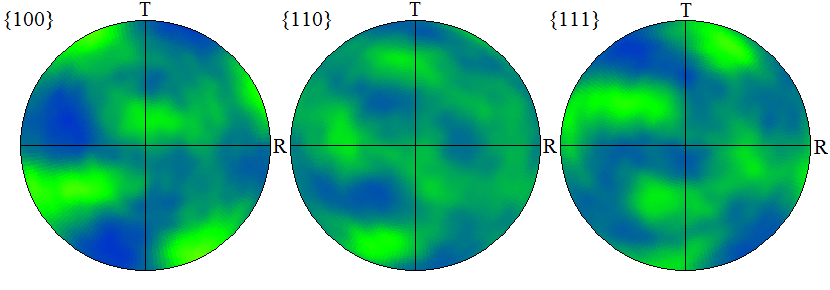
\includegraphics[width=1\columnwidth]{EDSBthickgaugeNuggetC2}}\hfill
		\subfigure{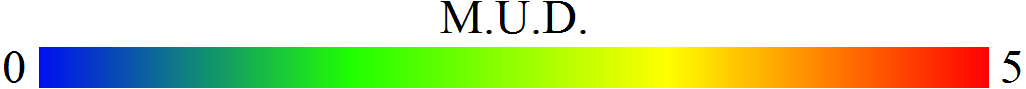
\includegraphics[width=.75\columnwidth]{EDSBScaleBar5}} \centering
		\caption{Upper hemisphere pole figures (equal area projection) from EBSD micro-texture measurements across the weld zone and over a range of gauge thickness. Where T is the short transverse direction and R is the rolling direction; the normal direction is orthogonal to the page. Multiples of uniform density (MUD) is indicative of the statistical distribution of crystal orientations within the sample.}
		\label{fig:EBSD}
	\end{figure*}	
	%    \newline\newline{\raggedright\textit{Influence of FSW on micro-texture}}
	%	\subsubsection{Influence of FSW on micro-texture}
	
	From figure \ref{fig:EBSD}, we can see that as-received material exhibits weak \{100\} fibre ($<100>$ parallel to the normal direction) in both the parent material and HAZ. In addition, both these regions of the weld also exhibit weak \{111\} rolled texture. The textures are described as weak because the mean uniform density peaks are less than 3 times random in the pole figures. Furthermore, the distribution of intensities in the \{110\} pole figure appears to be randomly distributed. In the TMAZ, the heavily distorted grains also exhibit weak \{100\} fibre, weak \{111\} rolled texture, and a random \{110\} texture. However, there exists a proportion of fine equiaxed grains  sampled within the TMAZ which, when analysed, exhibit a weak cube texture. The fine equiaxed grains within the nugget region of the weld exhibit a weak misoriented cube texture. It would appear that the welding process does not induce significant texture change with the exception of a subregion of grains in the TMAZ and the grains of the nugget. It is likely that the texture change is attributable to dynamic recrystallisation which is known to occur in the nugget. Since dynamic recrystallisation is a response to thermal input and plastic deformation, it is unsurprising that there is a subregion of recrystallised grains in the TMAZ. From these observations it is possible that texture development arising due to FSW may effect the measured mechanical properties of the nugget region. However, the effect is likely to be small due to the low intensities in the measured pole figures. 
	%	\subsubsection{Influence of material gauge thickness on micro-texture}
	%    \newline\newline{\raggedright\textit{Influence of material gauge thickness on micro-texture}}
	
	In both the thick and medium gauge (38 and 12.7 mm respectively), the as-received material demonstrates weak \{100\} fibre and weak \{111\} rolled texture; in all cases the peak intensity is approximately 2.5. The \{110\} texture appears randomly distributed in thick and medium gauge material. In contrast, the \{100\} and \{110\} pole figures of the thin gauge material show more distinct pole intensities compared with the thick and medium gauge material. However, in general the intensities remain relatively weak. Additionally, the \{111\} rolled texture is more distinct compared with the thick and medium gauge material. It is not unusual that texture becomes more distinct in thin gauge material as deformation during rolling causes alignment of the crystal grains. It must be noted that since only micro-texture measurements have been made, it is possible that the more distinct pole intensities is a localised effect. Studies of the macro scale texture using X-ray diffraction techniques may be able to determine if there texture variation is really significant with variation in gauge thickness of 2139-T8. In the context of this study, it is possible that by obtaining parameters for constitutive modelling (equation \ref{eq5}) separately from 2139-T8 material in different gauge thickness may be influenced by texture. There is likely to be some degree of anisotropy in the measured properties of the material. It is reasonable that for the purposes of modelling, the most conservative parameters be used from measuring the properties from the different material directions. Overall, the micro-texture of the material in thin gauges is still relatively weak compared to different alloys. 
	%	\begin{figure*}[h!t]	
	%		\subfigure[Base Metal (1.6 mm gauge thickness)]{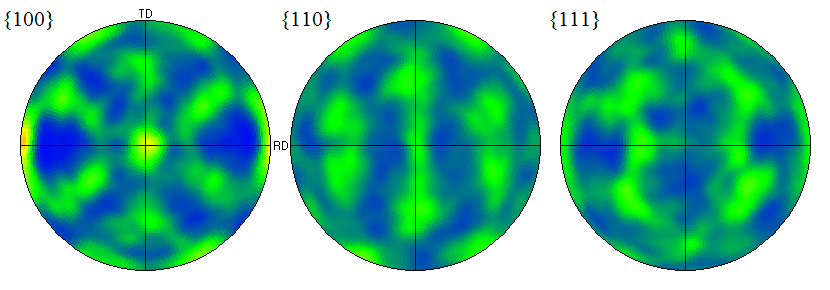
\includegraphics[width=1\columnwidth]{EDSBthingaugeC}} \hfill
	%		\subfigure[Base Metal (12.7 mm gauge thickness)]{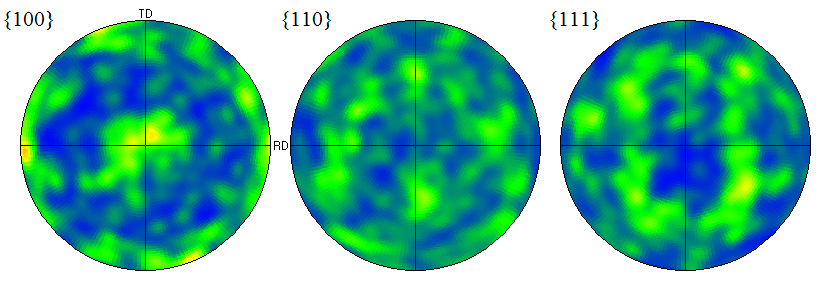
\includegraphics[width=1\columnwidth]{EDSBmediumgaugeC}}\hfill
	%		\subfigure[Base Metal (38 mm gauge thickness)]{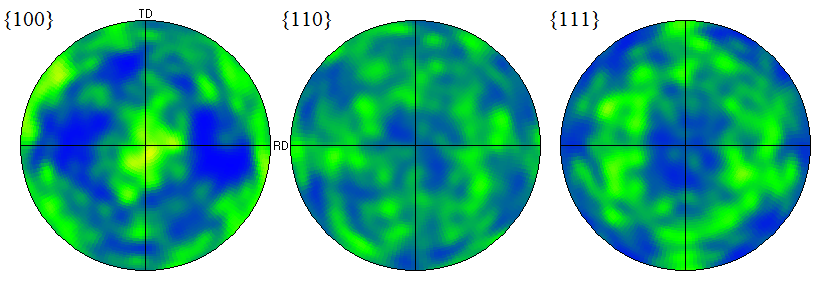
\includegraphics[width=1\columnwidth]{EDSBthickgaugeC}}\hfill
	%		\subfigure[HAZ (38 mm gauge thickness)]{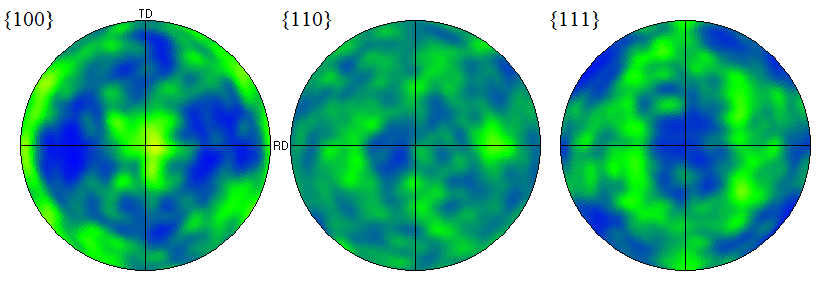
\includegraphics[width=1\columnwidth]{EDSBthickgaugeHAZC}}\hfill
	%		\subfigure[TMAZ (38 mm gauge thickness)]{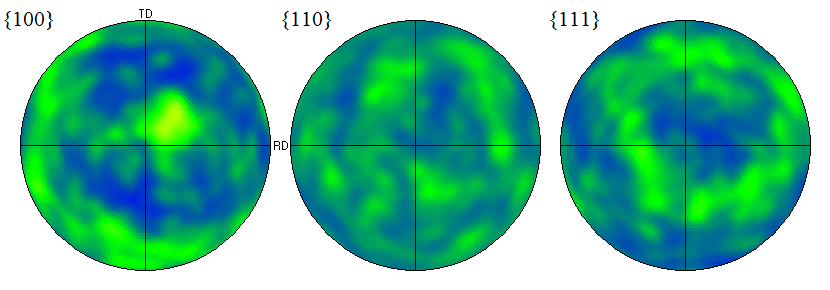
\includegraphics[width=1\columnwidth]{EDSBthickgaugeTMAZC}}\hfill
	%		\subfigure[Nugget (38 mm gauge thickness)]{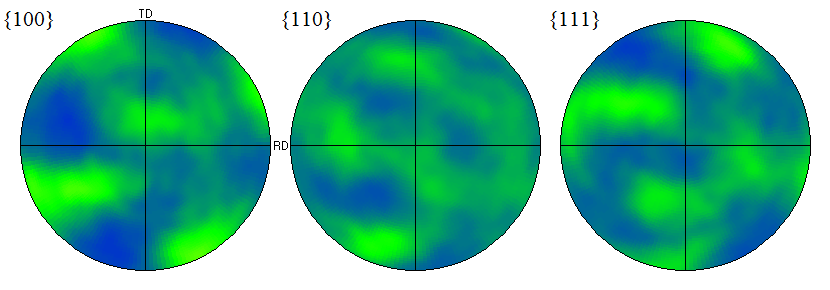
\includegraphics[width=1\columnwidth]{EDSBthickgaugeNuggetC}}\hfill
	%			\subfigure{\includegraphics[width=.75\columnwidth]{EDSBscalebar5}} \centering
	%		\caption{EBSD measurement of micro-texture across the weld zone and over a range of gauge thicknesses.}
	%		\label{fig:EBSD}
	%	\end{figure*}
	%	Describe what you see. Say that deformation and recrystallisation can be seen in the maps. Explain what textures there are - fibres etc. Say that this is also a limited study on gauge thickness because it is a micro-texture measurement. XRD is could be used to get a better understanding on macro scale texture development.
	%	Basically no change apart from nugget as expected. Varying gauge thickness may be problematic. Need to examine more large scale.
	%TODO Micro-texture Is this necessary? maybe. discuss with Joe/Phil
	%TODO Micro-texture say that there is exture development and in thin gauge material there is likely to be some anisotropy. This could impact on measurement of constitutive parameter. But if we use the worst case scenario for strain rate sensitivity, thermal sensitivity, we can obtain a conservative estimate for behaviour.
	
	%	\subsubsection{Summary}
	%	\label{RADMicrostructureSummary}
	%	The properties of 2139-T8 are widely reported to be dominated by the presence of the strengthening $\Omega$ phase. TEM observation of the $\Omega$ phase show that there is an extremely fine distribution of plate like precipitates oriented along the \{111$\}_\alpha$. The FSW process induces significant thermal loading allowing diffusional processes to alter the microstructure of the parent material. In the outer regions of the HAZ, the $\Omega$ phase appears to be over-aging as demonstrated by coarsening of the precipitates and an increase in the distribution of inter precipitate spacing. This is linked to the local thermal cycle and examination of the hardness distribution across the weld shows that this is a gradual process. Nevertheless, on a local scale, $\Omega$ phase remains finely distributed within the outer regions of the HAZ and is likely to remain the dominant contributor significantly to strengthening in the alloy. In the inner regions of the HAZ, TMAZ, and the nugget, temperatures are high enough to cause full dissolution of the $\Omega$ phase on a local scale. It is likely, therefore, that contributions from other sources of strengthening become relatively significant. It is conjectured that in these inner regions of the weld, solute strengthening and the formation of GP zones upon natural aging contribute towards the strength of the alloy. Furthermore, grain size analysis reveals that strengthening due to grain refinement may contribute to strengthening but is confined to the nugget region of the weld. TEM observations further reveal that there is a decrease in dislocation density from the parent material towards the centre of the weld. This is likely linked to recovery and recrystallisation processes which cause annihiliation of dislocations structures; this may influence the work hardening rate across the weld. Micro-texture analysis reveals that the nugget region has a random texture, which is distinct from any other region in the weld. All other regions retain the lightly rolled texture of the parent material and it is unlikely that texture variation in thick gauge material has a significant influence on the mechanical properties. However, anisotropy due to the texture in thin gauge materials may influence measured mechanical properties.
	\subsection{Mechanical Properties in simulated FSW}
	\label{RADMechProps}
	
	After measuring the mechanical response of simulated weld material, the parameters for a Johnson-Cook model were fitted for each region of the weld. Table \ref{tab:Mechprops} shows the distribution of properties across the weld region and figure \ref{fig:Mechprops} shows the measured mechanical response plotted alongside the Johnson-Cook model for the quasi-static regime. 
	
	The variation in yield stress in the outer regions of the HAZ appears to be in line with the literature as there is a constant linear relationship with hardness \cite{McWilliams2013,Grujicic2011a}; the linear coefficient is measured as 2.5. Furthermore, there is no significant variation in the measured work hardening rate as compared to the parent material in this outer region;  in both conditions it is measured at 0.4. 
	In the inner regions of the HAZ, there appears to be a slight variation in the linear relationship between yield stress and hardness; the linear coefficient reduces to 2.35. Additionally, there is a measured increase in work hardening rate which is approximately 0.5 in this region. 
	In the nugget region there is a more significant variation in the linear relationship of yield stress with hardness; the linear coefficient is measured to be 1.96. Furthermore, there is also a significant increase in work hardening rate which is approximately 0.65 in this region. 
	The measured data shows that the following assumptions for estimating the Johnson-Cook parameters across a weld using the lumped-mass method are not strictly true:
	\begin{enumerate}
		\item The linear relationship between yield stress and hardness is not constant across the weld. 
		\item The work hardening rate is not constant across the weld. 
	\end{enumerate}
	Both these relationships only appear to hold true in the outer regions of the weld but not in the inner regions of the weld. There is some variation in parameters across the weld appears to increase, but based on the limited number of data points, no particular relationship can be drawn. 
	
	\begin{figure}
		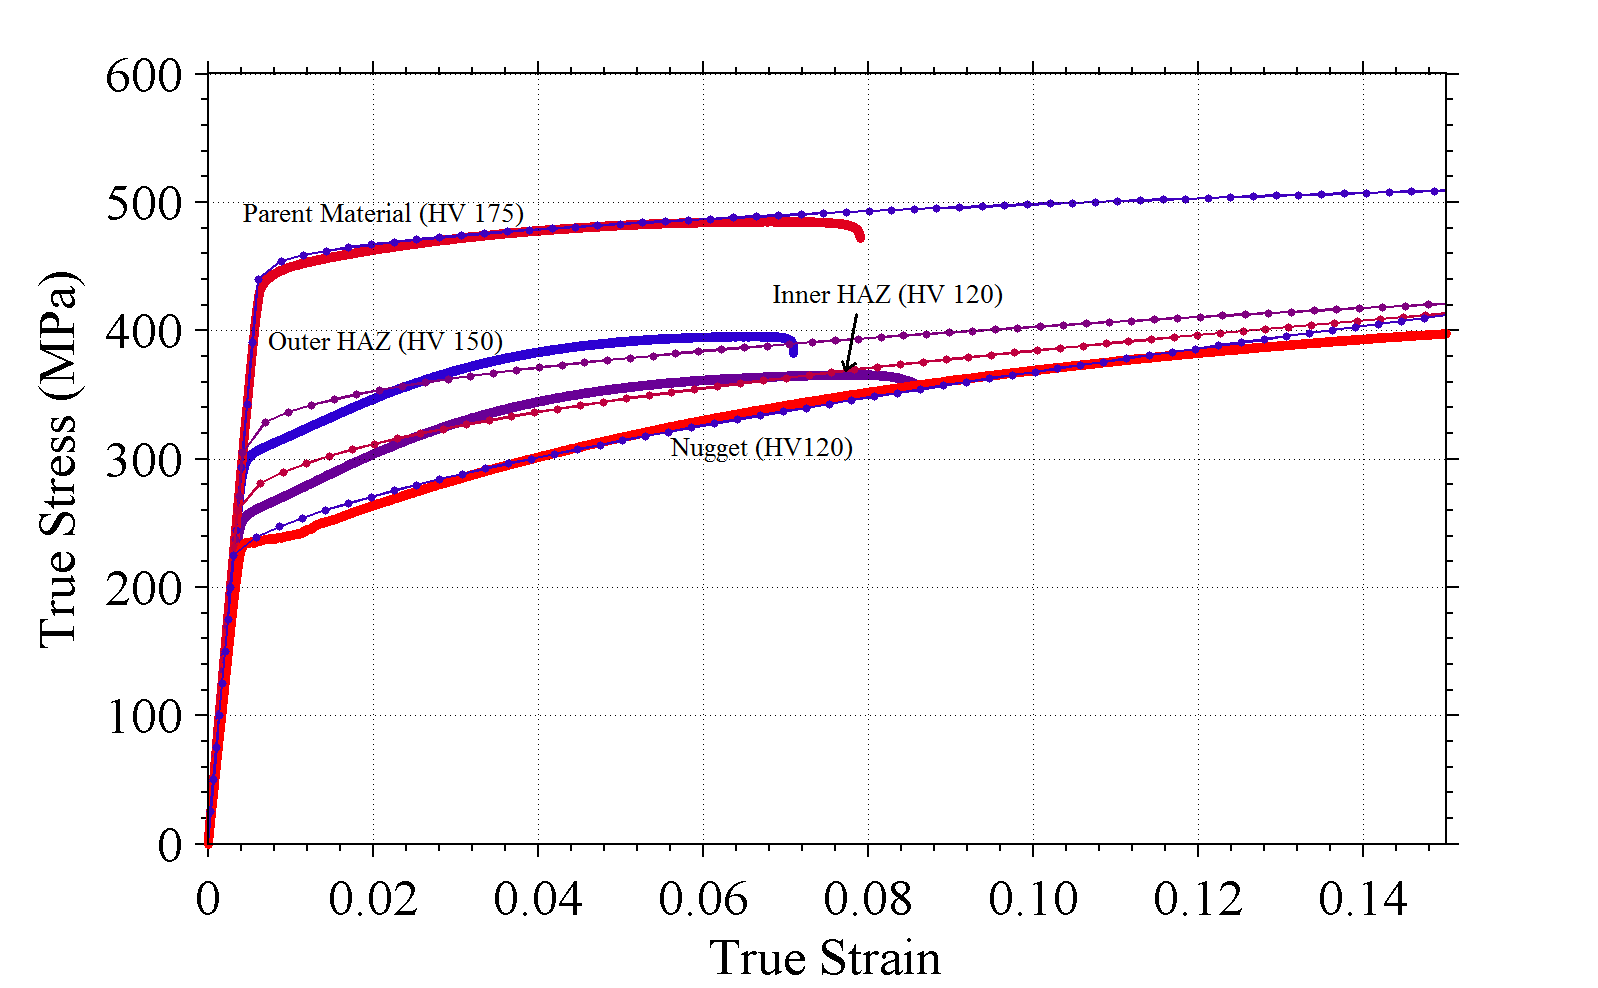
\includegraphics[width=1\linewidth]{MechPropBridgmansaltered} \hfill
		\caption{Example of measured mechanical property data for simulated weld material plotted alongside the Johnson-Cook prediction in the quasi-static regime; the Johnson-Cook models are plotted with dot markers.}
		\label{fig:Mechprops}
		%This figure was obtained by using a Bridgman factor to adjust tensile data. X-nug
	\end{figure}	
	%	\begin{figure}[h!t]
	%		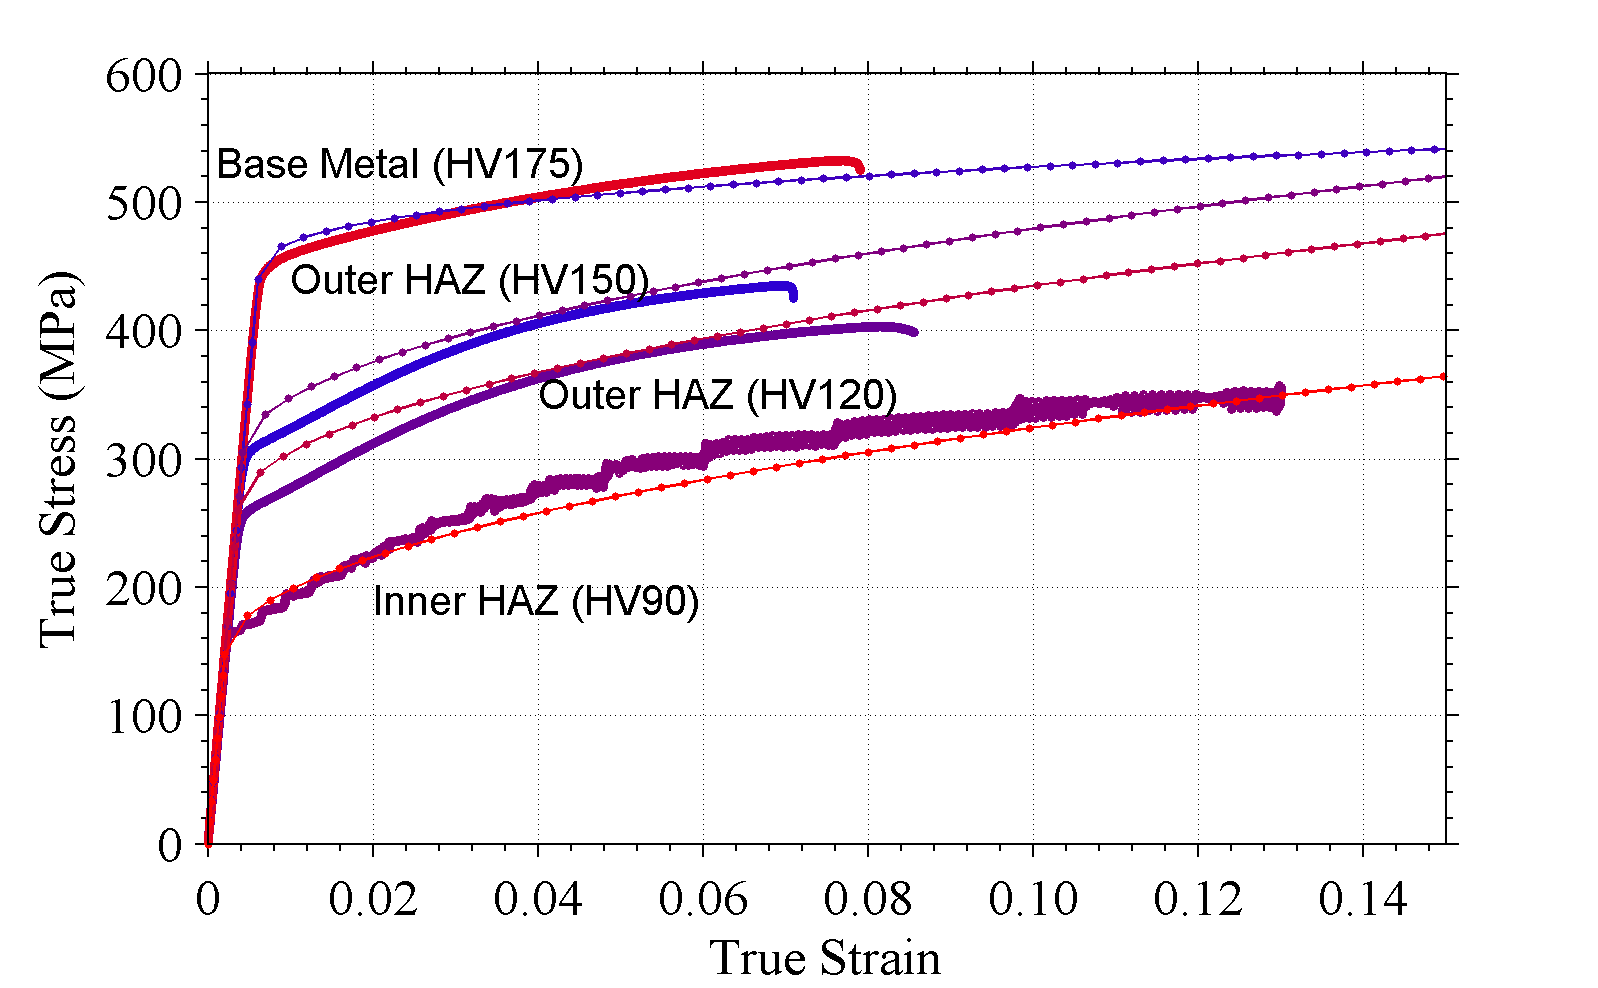
\includegraphics[width=1\linewidth]{ConstitutiveModelsaltered} \hfill
	%		\caption{Constitutive model prediction at quasi-static strain rates}
	%		\label{fig:Mechprops}
	%	\end{figure}
	%TODO Constitutive prediction should be in Part I. This should be fitted properties nevermind its not the right bloody parameters in the table (Hopefully the reviewers won't check)
	\begin{table}[h!]
		\centering
		\caption{Johnson-Cook parameters fitted to experimentally measured mechanical properties in the weld.}
		\resizebox{\columnwidth}{!}{%
			\begin{tabular}[c]{@{}ccccccc@{}} \toprule Region of weld & Hardness Vickers & k & B (MPa) & n & C & m \\ \midrule Base Metal & 175 & 2.5 & 250 & 0.4 & 0.02 & 1 \\ Outer HAZ & 150 & 2.5 & 250 & 0.4 & 0.02 & 1 \\ Inner HAZ & 120 & 2.35 & 400 & 0.5 & 0.03 & 1 \\ Nugget & 120 & 1.96 & 650 & 0.65 & 0.04 & 1\\ \bottomrule
			\end{tabular}
		}
		\label{tab:Mechprops}
	\end{table}

The measured strain rate sensitivity of 2139-T8 appears to correlate with data from Vural et al. who showed that the alloy remains strain rate insensitive until strain rates of the order $10^3\text{s}^{-1}$ \cite{Vural2009}. Furthermore, in the outer regions of the HAZ there was a negligible variation in strain rate sensitivity of the alloy. This insensitivity is thought to be due to the propagation dynamics of dislocations due to the geometry and alignment of the $\Omega$ phase in the matrix. Dislocations are thought to generate at the edge of the precipitate under deformation and propagate along the broad face of the $\Omega$ phase due to its alignment with the natural slip planes of aluminium forcing dislocations to shear through the precipitates. Unlike precipitates aligned with the $<100>$ direction, the precipitates aligned with $<111>$ will not undergo localised "buckling" of precipitates \cite{Elkhodary2010,Elkhodary2011b,Casem2009}. Hence, resistance to dislocation motion is retained in the presence of the $\Omega$ phase. In the inner regions of the HAZ and the nugget, where the $\Omega$ phase is in dissolution on a local scale, it is unsurprising that there is an increase in strain rate sensitivity. It is likely that strengthening arising from other strengthening phases are contributing to strength. Since they are aligned with directions not parallel to $<111>$ it likely that they will exhibit "buckling" at high strain rates and thereby become strain rate sensitive. Towards the centre of the weld any strengthening precipitates will be coarser and more susceptible to this behaviour. This could explain the increase in strain rate sensitivity across the weld.

In contrast, the measured thermal sensitivity reduces across the weld. This is expected since alloy strength is attributed to the $\Omega$ phase. As the volume fraction of precipitates reduces towards the weld centre, there is a reduction in yield strength as shown in table \ref{tab:Mechprops}. Therefore, the overall softening effect of and sensitivity to temperature will be reducing towards the centre of the weld.
	
	%TODO put in figure of property distribution across weld
	%	Here are the measured results A,B,n,C,m
	%	How does this compare with typical FE methods in literature (don't capture all variation)
	\subsection{Johnson-Cook constitutive parameter definition for aluminium 2139-T8 subjected to FSW}
	\label{RADJCModel}
	The properties of 2139-T8 are widely reported to be dominated by the presence of the strengthening $\Omega$ phase \cite{Cho2006}. TEM observation of the $\Omega$ phase show that there is an extremely fine distribution of plate like precipitates oriented along the \{111$\}_\alpha$ \cite{Cho2006,Bakavos2008}. The FSW process induces significant thermal loading allowing diffusional processes to alter the microstructure of the parent material \cite{Shercliff1990,Shercliff1990a}. In the outer regions of the HAZ, the $\Omega$ phase appears to be over-aging as demonstrated by coarsening of the precipitates and an increase in the distribution of inter precipitate spacing. This is linked to the local thermal cycle and examination of the hardness distribution across the weld shows that this is a gradual process. Nevertheless, on a local scale, $\Omega$ phase remains finely distributed within the outer regions of the HAZ and is likely to remain the dominant contributor significantly to strengthening in the alloy. 
	From the measured mechanical response of the parent material and the outer HAZ, there appears to be a constant linear relationship between yield stress and hardness. Furthermore, the work hardening rate remains relatively constant.
	
	In the inner regions of the HAZ, TMAZ, and the nugget, temperatures are high enough to cause full dissolution of the $\Omega$ phase on a local scale. It is likely, therefore, that contributions from other sources of strengthening become comparatively significant \cite{Shercliff1990a}. It is conjectured here that in these inner regions of the weld, solute strengthening and the formation of GP zones upon natural aging contribute towards the strength of the alloy \cite{Bakavos2008}. Furthermore, grain size analysis reveals that strengthening due to grain refinement may contribute to strengthening but is confined to the nugget region of the weld. TEM observations further reveal that there is a decrease in dislocation density from the parent material towards the centre of the weld. This is likely linked to recovery and recrystallisation processes which cause annihilation of dislocations structures. Furthermore, this is indicative of a possible influence on the work hardening rate across the weld. Indeed, the measured linear relationship between yield stress and hardness decreases distinctly in the inner HAZ and again in the nugget region. The measured work hardening rate increases distinctly in the inner HAZ and again in the nugget region.
	
	The observation from the limited number of data points suggests that distinct changes in mechanical properties are linked to distinct changes in microstructure. These microstructural changes are a function of both the thermal history and plastic deformation, which depends on the proximity to the welding tool. Hence, we can define piece-wise continuous constitutive model parameters across the weld zone using equations \ref{eq6}-\ref{eq11}.  
	\begin{equation}
	\label{eq6}
	A=k*Hv 
	\end{equation}
	\begin{equation}
	\label{eq7}
	B=\text{f}_1(T,t,\vec{\textbf{x}})
	\end{equation}
	\begin{equation}
	\label{eq8}
	n=\text{f}_2(T,t,\vec{\textbf{x}})
	\end{equation}
	\begin{equation}
	\label{eq9}
	C=\text{f}_3(T,t,\vec{\textbf{x}})
	\end{equation}
	\begin{equation}
	\label{eq10}
	m=\text{f}_4(T,t,\vec{\textbf{x}})
	\end{equation}
	Where
	\begin{equation}
	\label{eq11}
	k=\text{f}_5(T,t,\vec{\textbf{x}})
	\end{equation}
	and $\vec{\textbf{x}}$ is the position within the welded sample relative to the weld centreline.
	
	If we consider the quasi-static properties illustrated in figure \ref{fig:MechpropsVar}, and the hardness variation across FSW 2139-T8, the application of equations \ref{eq6}-\ref{eq11} is relatively simple. The first boundary defining the step changes in measured properties is the location where dissolution of precipitates is assumed to occur; this defines the start of the inner HAZ and coincides with the location of the minima of the ``W-shaped" post-weld hardness profile, as described in \S\ref{ModellingProcess}. The end of the inner HAZ is defined by the geometry of the welding tool pin; the nugget region is bounded by the dimensions of the tool. Hence, a method for defining Johson-Cook parameters across the weld is as follows:
	\begin{enumerate}
		\item Heat treat material to simulate distinct regions within the weld (Inner HAZ, Outer HAZ, and TMAZ) and generate representative nugget material from an actual weld.
		\item Measure the mechanical response of simulated material in the quasi-static, high strain rate, and high temperature regimes.
		\item Fit Johnson-Cook parameters to measured data for each region of the weld.
		\item Specify boundaries for defining material properties with piece-wise continuous functions (equations \ref{eq6}-\ref{eq11}) across the weld zone based on the location of precipitate dissolution and position relative to the tool geometry.
	\end{enumerate}  
	\begin{figure}
		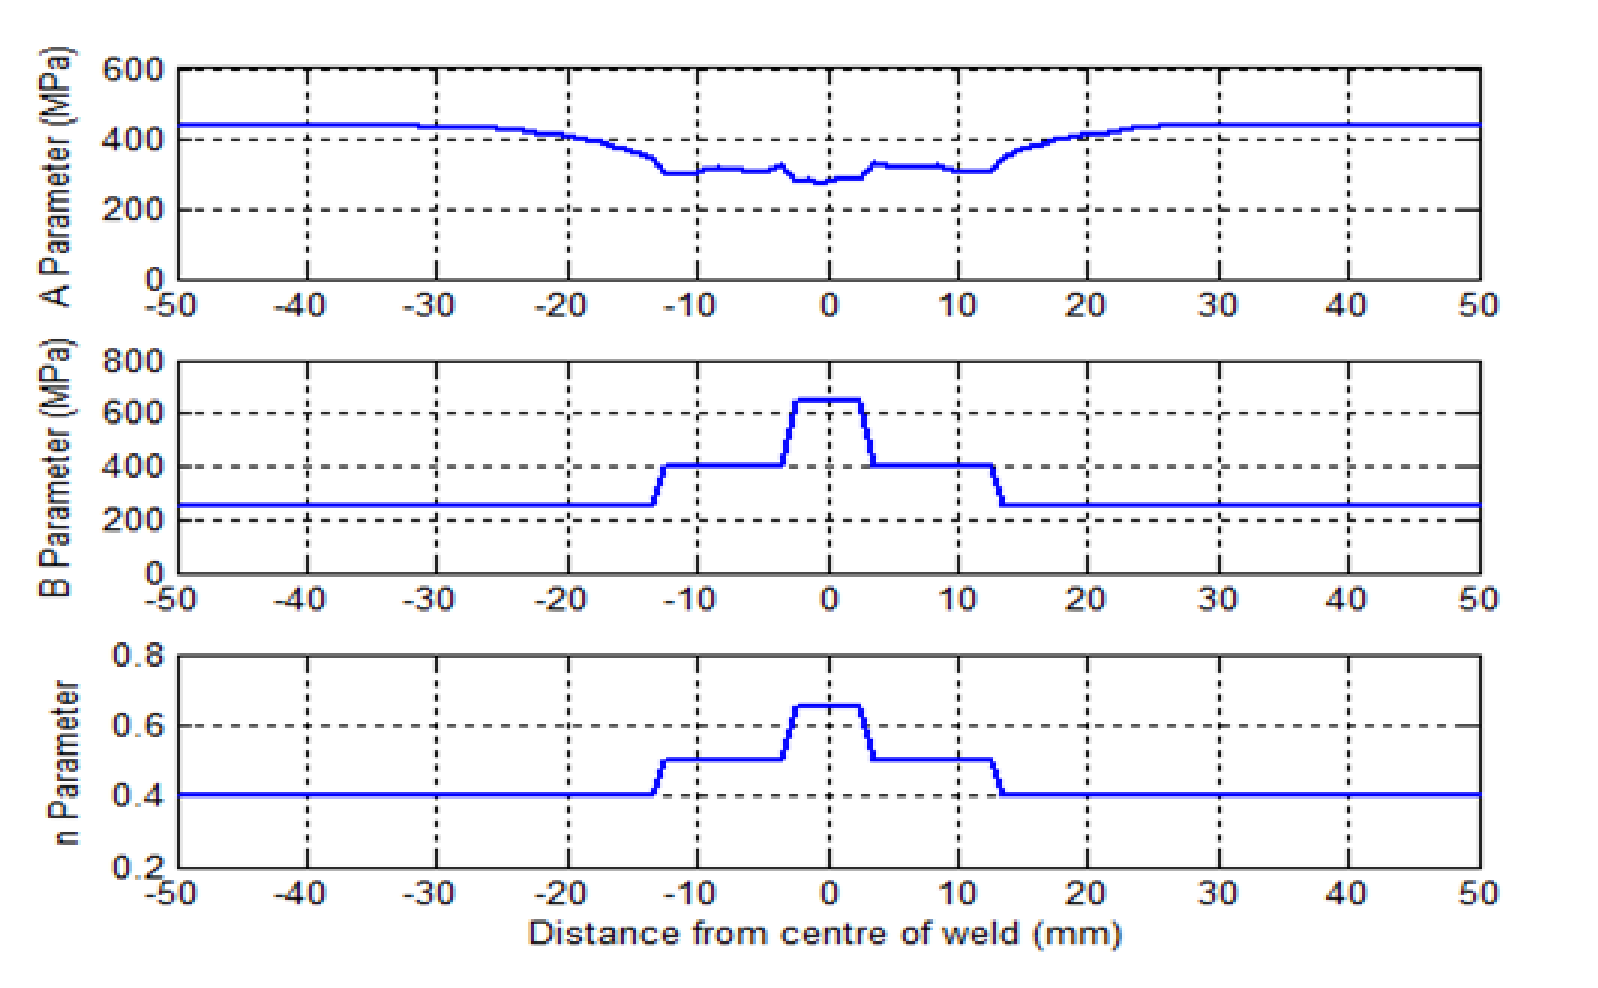
\includegraphics[width=1\linewidth]{PropertyVariation} 
		\caption{Proposed variation of the Johnson-Cook parameters across a weld cross section.}
		\label{fig:MechpropsVar}
		%This figure was obtained by using a Bridgman factor to adjust tensile data. X-nug
	\end{figure}	
	\begin{figure}
		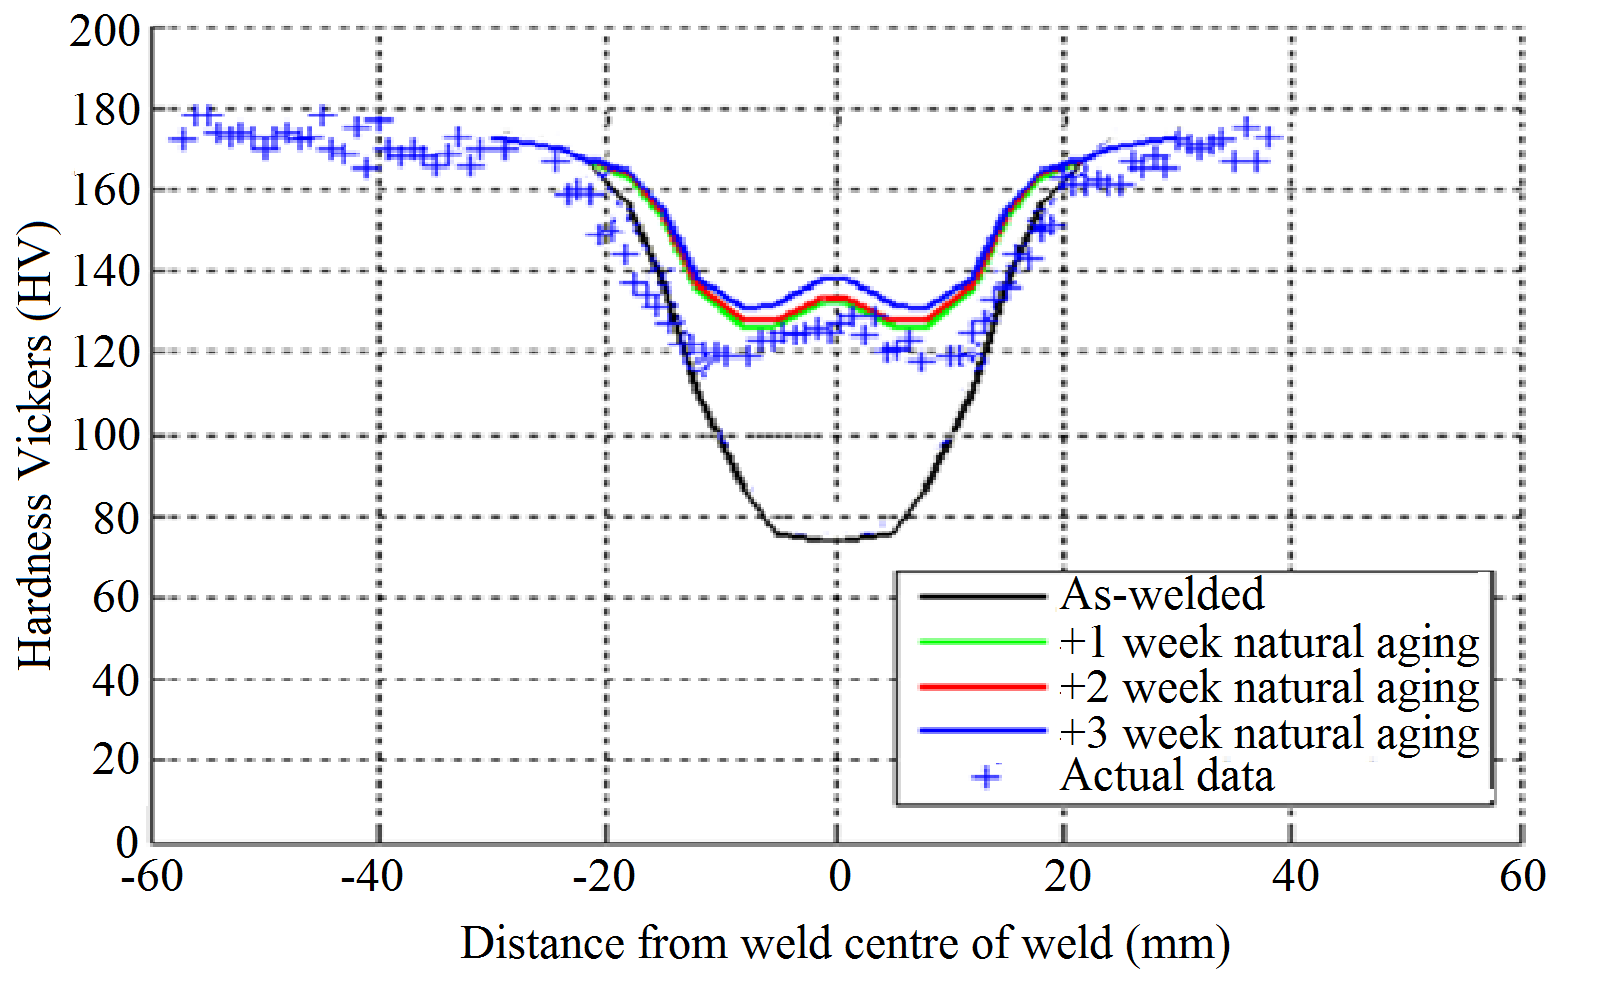
\includegraphics[width=1\linewidth]{HardnessVariation} 
		\caption{Proposed variation of the Johnson-Cook parameters across a weld cross section.}
		\label{fig:HardnessVar}
		%This figure was obtained by using a Bridgman factor to adjust tensile data. X-nug
	\end{figure}	
	
	%	You can decide how to partition effectively based on examination of hardness map and these simulated weld mech props
	\subsubsection{Limitations}
	The Johnson-Cook parameters for the weld regions of FSW 2139-T8 were obtained material in a range of gauge thickness'. 
	Micro-texture analysis reveals that thin gauge material has more distinct texture than thick gauge material as a consequence of deformation due to rolling during the manufacturing process. Examination of the pole figures in figure \ref{fig:EBSD} shows that the degree of texturing is relatively low as pole intensities are less than 3. Nonetheless, it is likely that anisotropy due to the texture in thin gauge materials influences the measured mechanical properties. A conservative approach would be to use directional parameters to determine an upper and lower bound of constitutive behaviour.
	
	%	Essentially, you are assuming that an equivalent softness is an equivalent microstructure. This is not necessarily true. However, since J-C models are an estimate of bulk properties, using simulated materials give a better indicator of bulk properties as it allows more effects of welding to be accounted for in obtaining material properties. Since existing methods assume no variation in critical properties of a weld, then accounting for them in some way leads to more accurate results. When extended to a structural model, you also eliminate errors from calibration of weld models. Hence, the improvement in accuracy.
	
	% % % % % % % % % % % % % % % % % % % % % % % % % % % % % % % % % % % % % % % % % % % % % % % % % %
	% % % % Conclusions
	% % % % % % % % % % % % % % % % % % % % % % % % % % % % % % % % % % % % % % % % % % % % % % % % % %
	\section{Conclusions}
	\label{Conclusion}
	In addition to predicting the hardness distribution for any welding parameters and tool dimensions, the Shercliff method can be used to heat treat 2139-T8 to simulate any region within the weld. This method was used to generate mechanical properties for the regions local to the weld. Data for a representative nugget region were obtained from nugget material extracted from a real weld. TEM and EBSD studies were carried out on actual FSW 2139-T8 in order to capture local microstructural variation across the weld. Based on these studies the following observations were made:
	
	\begin{enumerate}
		\item FSW induces significant variation to the local microstructure in aluminium 2139-T8. In the outer regions of the HAZ, precipitates undergo partial dissolution and coarsening but the strengthening $\Omega$ phase remains the greatest contributor to alloy strengthening. In these regions the measured work hardening rate and the linear relationship of yield stress with hardness is close to the parent material. The dissolution of precipitates in this region is a gradual process which is dependent on the local thermal history from the weld. 
		
		\item In the inner regions of the HAZ and TMAZ, temperatures are high enough to cause full dissolution of $\Omega$ phase. Hence, other contributions to alloy strength influence the measured material properties, such as solute stregnthening and the formation of GP zones upon natural aging. In these regions, the work hardening rate increases distinctly compared with the parent material and outer HAZ. Furthermore, there is a distinct decrease in the linear relationship of yield stress with hardness compared with the parent material and outer HAZ. The position in the weld where precipitates undergo full dissolution can be predicted using the Shercliff method and corresponds to the minima of the typical ``W-shape" hardness profile of the weld.
		
		\item In the nugget region, the combination of plastic deformation and transient temperature rise due to interaction with the weld tool has led to dynamic recrystallisation of the aluminium matrix in addition to causing full local dissolution of the $\Omega$ phase. In this region of the weld, the contribution to alloy strengthening which affects material properties is due to solute strengthening, the formation of GP zones upon natural aging and grain refinement. In this region, the measured work hardening rate demonstrates a distinct increase compared with the other regions of the weld. Furthermore, there is a distinct decrease in the linear relationship of yield stress with hardness. The position in the weld that can be classified as weld nugget is encapsulated approximately by the dimensions of the welding tool pin.
		
		\item These observation indicate that the typical assumptions in the ``lumped-mass" approach for constitutive modelling does not capture significant property variation in welded material. Hence, we suggest piece-wise continuous functions based on measurements of representative weld material to capture distinct changes in properties across the weld.
	\end{enumerate}
	
	Based on these observations, the Johnson-Cook parameters can be defined for any welding conditions from the measured properties of ``simulated" weld material, observation of the hardness distribution of the weld, and the dimensions of the welding tool. It must be noted that micro-texture analysis reveals that anisotropy in material properties due to texture development is likely to influence the properties of thin gauge material. Therefore, simply defining Johnson-Cook parameters based on our observations is likely to be subject to some degree of error. Conservative parameters should be used to define upper and lower bounds of material response.
	
	
	% % % % % % % % % % % % % % % % % % % % % % % % % % % % % % % % % % % % % % % % % % % % % % % % % %
	% % % % Acknowledgements
	% % % % % % % % % % % % % % % % % % % % % % % % % % % % % % % % % % % % % % % % % % % % % % % % % %
	\section*{Acknowledgements}
	\label{Acknowledgements}
	The authors acknowledge the funding granted from EPSRC via the Advanced Metallic Systems CDT (EP/L016273/1) at the Universities of Manchester and Sheffield and LATEST2 program (EP/G022402/1). Further, the authors acknowledge DSTL for their contribution towards development of the FE method; Constellium for the provision and manufacture of materials; and Blastech for technical support during blast testing. Thanks also to David Strong and Bill Storrey for their contribution towards experimental testing; and Samuel Tammas-Williams, Tom$\acute{\text{a}}$s Brownsmith, and Richard Watson for their assistance in producing this paper. Please contact the corresponding author for access to the original data used in this article.
	
	
	% % % % % % % % % % % % % % % % % % % % % % % % % % % % % % % % % % % % % % % % % % % % % % % % % %
	% % % % References
	% % % % % % % % % % % % % % % % % % % % % % % % % % % % % % % % % % % % % % % % % % % % % % % % % %
	\section*{References}
	\bibliographystyle{elsarticle-num} 
	%Referencing system for in the office....
	\bibliography{C:/Users/mbgm6aab/Documents/AdvancedMetallicSystemsCDT/PhD/Papers/library}
	%Referencing system for home....
	%\bibliography{C:/Users/Public/Documents/AdvancedMetallicSystemsCDT/PhD/Papers/library}
	
	
	%% else use the following coding to input the bibitems directly in the
	%% TeX file.
	
	%\begin{thebibliography}{00}
	
	%% \bibitem{label}
	%% Text of bibliographic item
	
	%\bibitem{}
	
	%\end{thebibliography}
\end{document}
\endinput
%%
%% End of file `elsarticle-template-num.tex'.
